% Created by tikzDevice version 0.12.6 on 2024-11-25 07:15:47
% !TEX encoding = UTF-8 Unicode
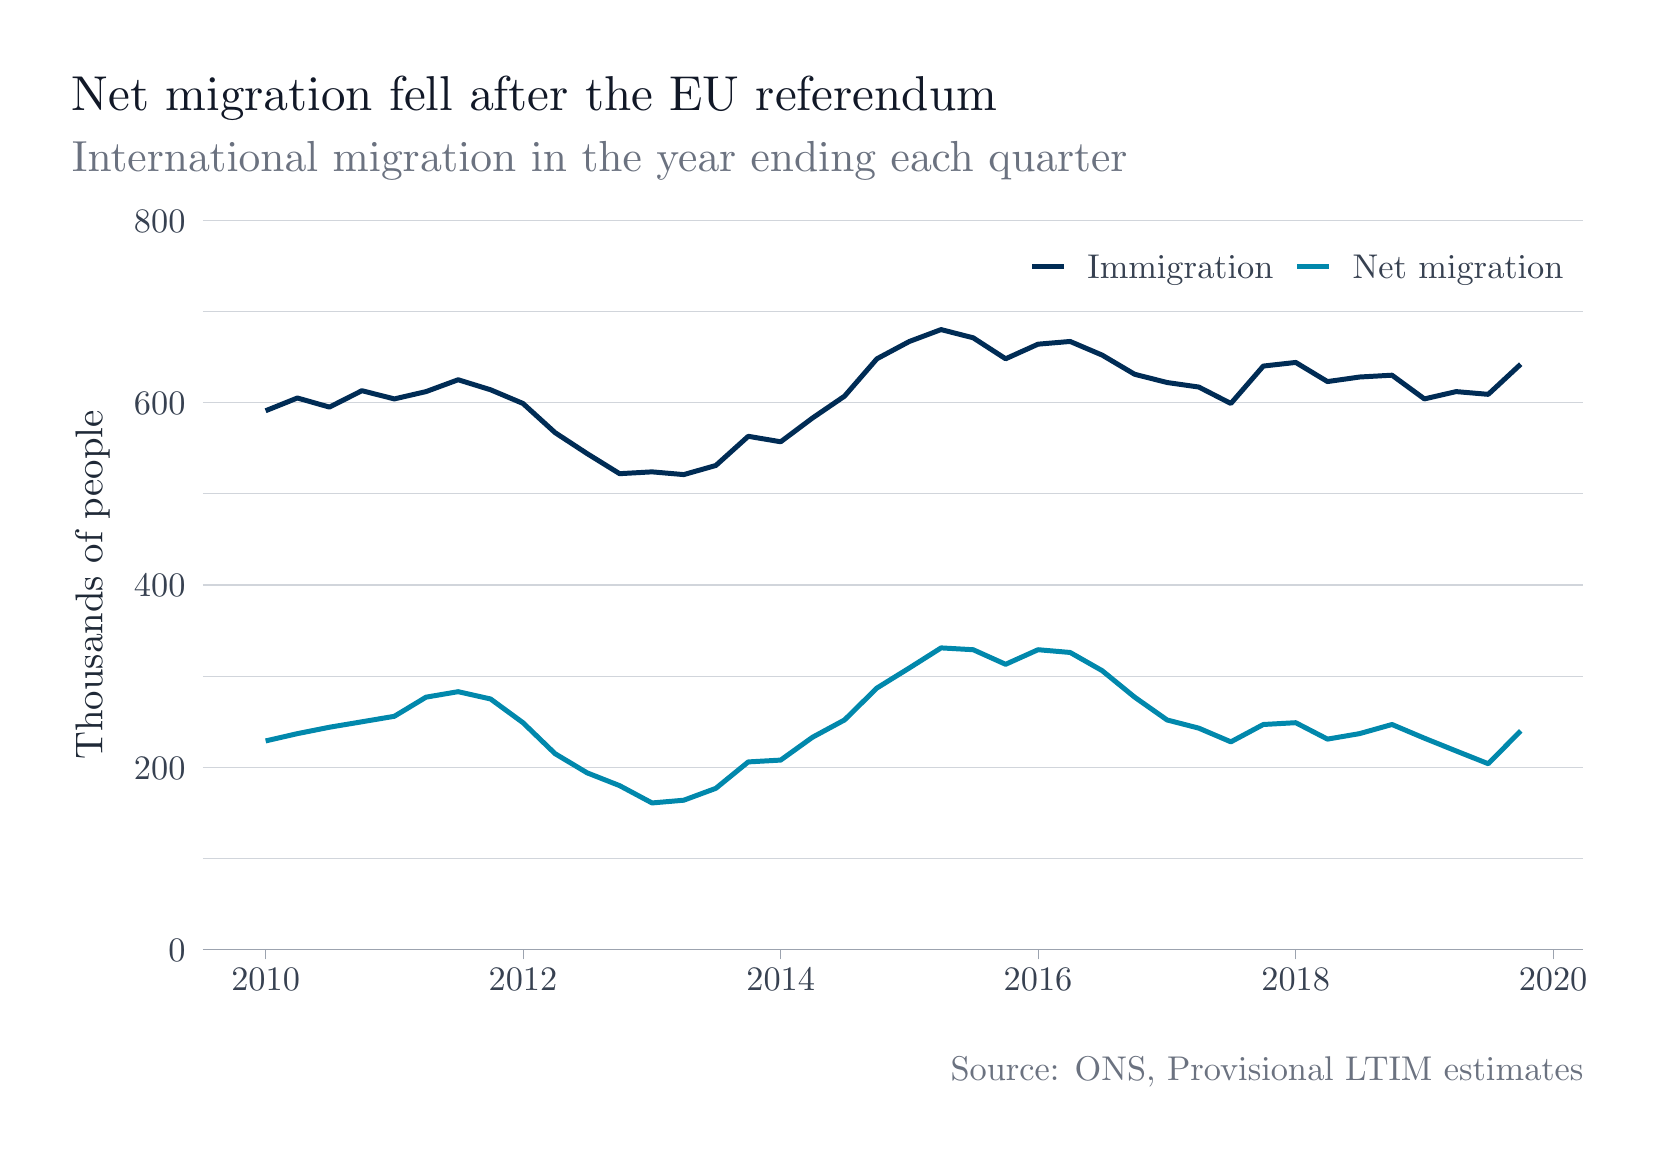
\begin{tikzpicture}[x=1pt,y=1pt]
\definecolor{fillColor}{RGB}{255,255,255}
\path[use as bounding box,fill=fillColor] (0,0) rectangle (578.16,397.48);
\begin{scope}
\path[clip] (  0.00,  0.00) rectangle (578.16,397.48);
\definecolor{drawColor}{RGB}{255,255,255}

\path[draw=drawColor,line width= 0.7pt,line join=round,line cap=round,fill=fillColor] (  0.00,  0.00) rectangle (578.16,397.48);
\end{scope}
\begin{scope}
\path[clip] ( 63.32, 64.27) rectangle (562.16,327.93);
\definecolor{drawColor}{RGB}{255,255,255}
\definecolor{fillColor}{RGB}{255,255,255}

\path[draw=drawColor,line width= 0.7pt,line join=round,line cap=round,fill=fillColor] ( 63.32, 64.27) rectangle (562.16,327.93);
\definecolor{drawColor}{RGB}{209,213,219}

\path[draw=drawColor,line width= 0.4pt,line join=round] ( 63.32, 97.23) --
	(562.16, 97.23);

\path[draw=drawColor,line width= 0.4pt,line join=round] ( 63.32,163.14) --
	(562.16,163.14);

\path[draw=drawColor,line width= 0.4pt,line join=round] ( 63.32,229.06) --
	(562.16,229.06);

\path[draw=drawColor,line width= 0.4pt,line join=round] ( 63.32,294.97) --
	(562.16,294.97);

\path[draw=drawColor,line width= 0.4pt,line join=round] ( 63.32, 64.27) --
	(562.16, 64.27);

\path[draw=drawColor,line width= 0.4pt,line join=round] ( 63.32,130.19) --
	(562.16,130.19);

\path[draw=drawColor,line width= 0.4pt,line join=round] ( 63.32,196.10) --
	(562.16,196.10);

\path[draw=drawColor,line width= 0.4pt,line join=round] ( 63.32,262.01) --
	(562.16,262.01);

\path[draw=drawColor,line width= 0.4pt,line join=round] ( 63.32,327.93) --
	(562.16,327.93);
\definecolor{drawColor}{RGB}{0,44,85}

\path[draw=drawColor,line width= 1.8pt,line join=round] ( 85.99,259.05) --
	( 97.46,263.66) --
	(109.05,260.37) --
	(120.77,266.30) --
	(132.49,263.33) --
	(143.95,265.97) --
	(155.55,270.25) --
	(167.27,266.63) --
	(178.98,261.68) --
	(190.58,251.14) --
	(202.17,243.56) --
	(213.89,236.31) --
	(225.61,236.97) --
	(237.07,235.98) --
	(248.66,239.27) --
	(260.38,249.82) --
	(272.10,247.84) --
	(283.57,256.41) --
	(295.16,264.32) --
	(306.88,277.83) --
	(318.60,284.09) --
	(330.06,288.38) --
	(341.66,285.41) --
	(353.38,277.83) --
	(365.09,283.11) --
	(376.69,284.09) --
	(388.28,279.15) --
	(400.00,272.23) --
	(411.72,269.26) --
	(423.18,267.62) --
	(434.77,261.68) --
	(446.49,275.20) --
	(458.21,276.51) --
	(469.68,269.59) --
	(481.27,271.24) --
	(492.99,271.90) --
	(504.71,263.33) --
	(516.17,265.97) --
	(527.77,264.98) --
	(539.49,275.86);
\definecolor{drawColor}{RGB}{1,136,172}

\path[draw=drawColor,line width= 1.8pt,line join=round] ( 85.99,139.74) --
	( 97.46,142.38) --
	(109.05,144.69) --
	(120.77,146.66) --
	(132.49,148.64) --
	(143.95,155.56) --
	(155.55,157.54) --
	(167.27,154.90) --
	(178.98,146.33) --
	(190.58,135.13) --
	(202.17,128.21) --
	(213.89,123.59) --
	(225.61,117.33) --
	(237.07,118.32) --
	(248.66,122.61) --
	(260.38,132.16) --
	(272.10,132.82) --
	(283.57,141.06) --
	(295.16,147.32) --
	(306.88,158.86) --
	(318.60,166.11) --
	(330.06,173.36) --
	(341.66,172.70) --
	(353.38,167.43) --
	(365.09,172.70) --
	(376.69,171.71) --
	(388.28,165.12) --
	(400.00,155.56) --
	(411.72,147.32) --
	(423.18,144.36) --
	(434.77,139.41) --
	(446.49,145.68) --
	(458.21,146.33) --
	(469.68,140.40) --
	(481.27,142.38) --
	(492.99,145.68) --
	(504.71,140.73) --
	(516.17,136.12) --
	(527.77,131.50) --
	(539.49,143.37);
\end{scope}
\begin{scope}
\path[clip] (  0.00,  0.00) rectangle (578.16,397.48);
\definecolor{drawColor}{RGB}{55,65,81}

\node[text=drawColor,anchor=base east,inner sep=0pt, outer sep=0pt, scale=  1.24] at ( 57.02, 59.99) {0};

\node[text=drawColor,anchor=base east,inner sep=0pt, outer sep=0pt, scale=  1.24] at ( 57.02,125.90) {200};

\node[text=drawColor,anchor=base east,inner sep=0pt, outer sep=0pt, scale=  1.24] at ( 57.02,191.82) {400};

\node[text=drawColor,anchor=base east,inner sep=0pt, outer sep=0pt, scale=  1.24] at ( 57.02,257.73) {600};

\node[text=drawColor,anchor=base east,inner sep=0pt, outer sep=0pt, scale=  1.24] at ( 57.02,323.64) {800};
\end{scope}
\begin{scope}
\path[clip] (  0.00,  0.00) rectangle (578.16,397.48);
\definecolor{drawColor}{RGB}{156,163,175}

\path[draw=drawColor,line width= 0.3pt,line join=round] ( 63.32, 64.27) --
	(562.16, 64.27);
\end{scope}
\begin{scope}
\path[clip] (  0.00,  0.00) rectangle (578.16,397.48);
\definecolor{drawColor}{RGB}{156,163,175}

\path[draw=drawColor,line width= 0.3pt,line join=round] ( 85.99, 60.77) --
	( 85.99, 64.27);

\path[draw=drawColor,line width= 0.3pt,line join=round] (178.98, 60.77) --
	(178.98, 64.27);

\path[draw=drawColor,line width= 0.3pt,line join=round] (272.10, 60.77) --
	(272.10, 64.27);

\path[draw=drawColor,line width= 0.3pt,line join=round] (365.09, 60.77) --
	(365.09, 64.27);

\path[draw=drawColor,line width= 0.3pt,line join=round] (458.21, 60.77) --
	(458.21, 64.27);

\path[draw=drawColor,line width= 0.3pt,line join=round] (551.20, 60.77) --
	(551.20, 64.27);
\end{scope}
\begin{scope}
\path[clip] (  0.00,  0.00) rectangle (578.16,397.48);
\definecolor{drawColor}{RGB}{55,65,81}

\node[text=drawColor,anchor=base,inner sep=0pt, outer sep=0pt, scale=  1.24] at ( 85.99, 49.40) {2010};

\node[text=drawColor,anchor=base,inner sep=0pt, outer sep=0pt, scale=  1.24] at (178.98, 49.40) {2012};

\node[text=drawColor,anchor=base,inner sep=0pt, outer sep=0pt, scale=  1.24] at (272.10, 49.40) {2014};

\node[text=drawColor,anchor=base,inner sep=0pt, outer sep=0pt, scale=  1.24] at (365.09, 49.40) {2016};

\node[text=drawColor,anchor=base,inner sep=0pt, outer sep=0pt, scale=  1.24] at (458.21, 49.40) {2018};

\node[text=drawColor,anchor=base,inner sep=0pt, outer sep=0pt, scale=  1.24] at (551.20, 49.40) {2020};
\end{scope}
\begin{scope}
\path[clip] (  0.00,  0.00) rectangle (578.16,397.48);
\definecolor{drawColor}{RGB}{31,41,55}

\node[text=drawColor,rotate= 90.00,anchor=base,inner sep=0pt, outer sep=0pt, scale=  1.40] at ( 27.00,196.10) {Thousands of people};
\end{scope}
\begin{scope}
\path[clip] (  0.00,  0.00) rectangle (578.16,397.48);
\definecolor{drawColor}{RGB}{255,255,255}
\definecolor{fillColor}{RGB}{255,255,255}

\path[draw=drawColor,line width= 0.7pt,line join=round,line cap=round,fill=fillColor] (354.47,296.84) rectangle (562.16,325.29);
\end{scope}
\begin{scope}
\path[clip] (  0.00,  0.00) rectangle (578.16,397.48);
\definecolor{drawColor}{RGB}{255,255,255}
\definecolor{fillColor}{RGB}{255,255,255}

\path[draw=drawColor,line width= 0.7pt,line join=round,line cap=round,fill=fillColor] (361.47,303.84) rectangle (375.92,318.29);
\end{scope}
\begin{scope}
\path[clip] (  0.00,  0.00) rectangle (578.16,397.48);
\definecolor{drawColor}{RGB}{0,44,85}

\path[draw=drawColor,line width= 1.8pt,line join=round] (362.91,311.06) -- (374.48,311.06);
\end{scope}
\begin{scope}
\path[clip] (  0.00,  0.00) rectangle (578.16,397.48);
\definecolor{drawColor}{RGB}{255,255,255}
\definecolor{fillColor}{RGB}{255,255,255}

\path[draw=drawColor,line width= 0.7pt,line join=round,line cap=round,fill=fillColor] (457.32,303.84) rectangle (471.78,318.29);
\end{scope}
\begin{scope}
\path[clip] (  0.00,  0.00) rectangle (578.16,397.48);
\definecolor{drawColor}{RGB}{1,136,172}

\path[draw=drawColor,line width= 1.8pt,line join=round] (458.77,311.06) -- (470.33,311.06);
\end{scope}
\begin{scope}
\path[clip] (  0.00,  0.00) rectangle (578.16,397.48);
\definecolor{drawColor}{RGB}{55,65,81}

\node[text=drawColor,anchor=base west,inner sep=0pt, outer sep=0pt, scale=  1.24] at (382.92,306.78) {Immigration};
\end{scope}
\begin{scope}
\path[clip] (  0.00,  0.00) rectangle (578.16,397.48);
\definecolor{drawColor}{RGB}{55,65,81}

\node[text=drawColor,anchor=base west,inner sep=0pt, outer sep=0pt, scale=  1.24] at (478.78,306.78) {Net migration};
\end{scope}
\begin{scope}
\path[clip] (  0.00,  0.00) rectangle (578.16,397.48);
\definecolor{drawColor}{RGB}{107,114,128}

\node[text=drawColor,anchor=base west,inner sep=0pt, outer sep=0pt, scale=  1.57] at ( 16.00,345.46) {International migration in the year ending each quarter};
\end{scope}
\begin{scope}
\path[clip] (  0.00,  0.00) rectangle (578.16,397.48);
\definecolor{drawColor}{RGB}{17,24,39}

\node[text=drawColor,anchor=base west,inner sep=0pt, outer sep=0pt, scale=  1.77] at ( 16.00,367.56) {Net migration fell after the EU referendum};
\end{scope}
\begin{scope}
\path[clip] (  0.00,  0.00) rectangle (578.16,397.48);
\definecolor{drawColor}{RGB}{107,114,128}

\node[text=drawColor,anchor=base east,inner sep=0pt, outer sep=0pt, scale=  1.24] at (562.16, 17.21) {Source: ONS, Provisional LTIM estimates};
\end{scope}
\end{tikzpicture}
